

\subsection{Conclusion}

Realizamos este trabajo con el fin de poder optimizar temporalmente, mediante cambios en las implementaciones o compiladores, los filtros realizados. Podemos resumir nuestros resultados en este cuadro.


\begin{figure}[H]
\begin{center}
\minipage{0.8\textwidth}
  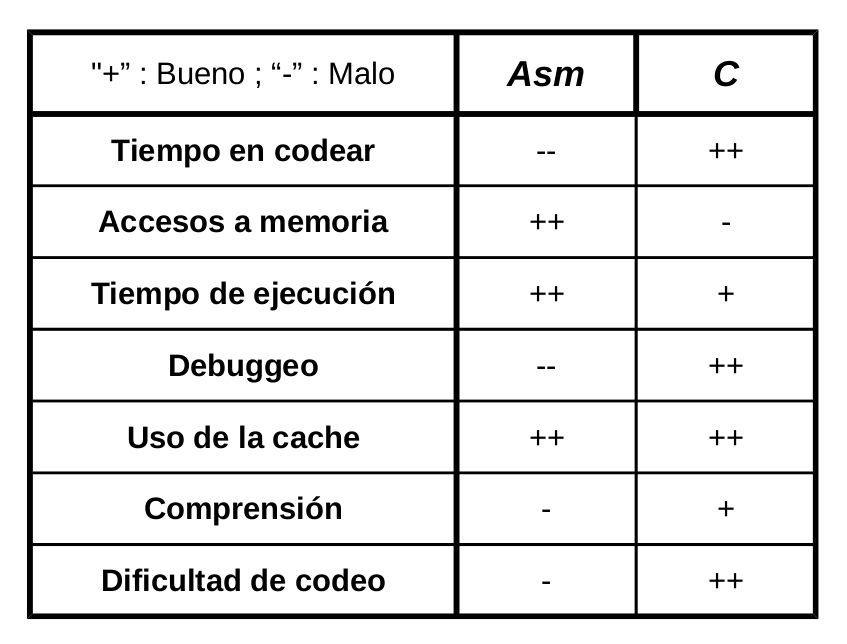
\includegraphics[width=\linewidth]{conclusion/conclusion.png}
\endminipage
\end{center}
\end{figure}

Basicamente, como concluimos que las implementaciones en assembler con simd son las optimas. Esto, siempre y cuando se apliquen sobre imagenes muy grandes o sobre un conjunto grande de imagenes. Esto se debe a los altos costes de implementacion que tiene asm (costes en terminos temporales). Sobre las difencias temporales entre asm y C podemos concluir que no se deben a la manera de manejar la cache.